%%=============================================================================
%% Inleiding
%%=============================================================================

\chapter{\IfLanguageName{dutch}{Inleiding}{Introduction}}
\label{ch:inleiding}

%De inleiding moet de lezer net genoeg informatie verschaffen om het onderwerp te begrijpen en in te zien waarom de onderzoeksvraag de moeite waard is om te onderzoeken. In de inleiding ga je literatuurverwijzingen beperken, zodat de tekst vlot leesbaar blijft. Je kan de inleiding verder onderverdelen in secties als dit de tekst verduidelijkt. Zaken die aan bod kunnen komen in de inleiding~:
%
%\begin{itemize}
%  \item context, achtergrond
%  \item afbakenen van het onderwerp
%  \item verantwoording van het onderwerp, methodologie
%  \item probleemstelling
%  \item onderzoeksdoelstelling
%  \item onderzoeksvraag
%  \item \ldots
%\end{itemize}

\section{Begrippen}
\label{sec:begrippen}

In deze bachelorproef wordt vaak gebruikt gemaakt van vakjargon. Hier worden belangrijke begrippen die vaak terugkomen uitgelegd.

\subsection{Artificiële Intelligentie (AI)}
\label{subsec:begrippen-ai}

Artificiële intelligentie of kunstmatige intelligentie is een verzamelnaam voor verschillende technologieën waarbij machines denken en handelen zoals mensen. AI is enorm breed en heeft verschillende hedendaagse toepassingen. Denk maar aan persoonlijke assistenten, spam detection, gps’en waarbij rekening gehouden wordt met ongevallen en files, zelfrijdende wagens, robots, aanbevelingen bij online shoppen, games spelen tegen computers, etc \autocite{Fagella2020}.

\subsection{Machine Learning (ML)}
\label{subsec:begrippen-ml}


Machine Learning of machinaal leren is een onderdeel van artificiële intelligentie waarbij computers zelfstandig leren van data en op die manier slimmer worden zonder dat mensen ze zelf slimmer gaan programmeren. Machines kunnen op basis van data hun eigen algoritmes veranderen en verbeteren. Een voorbeeld van machine learning is correctie bij het typen van documenten in Word. Mensen maken vaak typfouten, maar meestal zal Word zelf aangeven dat een woord fout is en een correct alternatief aanbieden. Dat gebeurt allemaal op basis van machine learning waarbij algoritmes de woorden en de context van de woorden gaan achterhalen en op die manier proberen een alternatief aan te bieden indien het woord onbekend is. Deze algoritmes leren ook telkens maar bij door eerdere correcties.


Volgens \textcite{Lievens2019} kan machinaal leren onderverdeeld worden in drie types:

\begin{itemize}
    \item \textbf{Gesuperviseerd leren:} \\
    
    Bij een algoritme voor gesuperviseerd leren zijn de input en (gewenste) output gegeven. Het is de bedoeling dat de algoritmes een samenhang tussen input en output vinden en zo een functie ontwerpen waarbij je bij een input de gewenste output krijgt. Zo kunnen voorspellingen gedaan worden. \\
    
    \item \textbf{Ongesuperviseerd leren:} \\
    
    Deze algoritmes gaan zelf op zoek naar informatie en structuur in een dataset zonder de gewenste output te krijgen. Ongesuperviseerd leren kan meer complexe taken oplossen dan gesuperviseerd leren, maar is wel onvoorspelbaarder en moeilijker om een betrouwbaar model te bekomen. \\
    
    \item \textbf{Reinforcement learning:} \\
    
    Deze techniek gaat niet werken met een dataset in tegenstelling tot de andere technieken die besproken zijn. Bij reinforcement learning wordt gewerkt met beloningen. Als een agent een goede actie uitvoert, dan wordt bij beloond en als hij iets slechts doet, krijgt hij een negatief signaal. Op basis van eerdere signalen zal het model slimmer worden en zich verder ontwikkelen. De doelstelling is de beloningen maximaliseren. \\
\end{itemize}

Chatbots behoren tot de categorie gesuperviseerd leren, omdat ze op basis van een dataset getraind worden om bepaalde acties te herkennen en uit te voeren. De andere types machine learning zullen niet verder besproken worden in deze bachelorproef.

\subsection{Chatbot}
\label{subsec:begrippen-chatbot}

Een chatbot of chatterbot is een samenvoeging van de woorden chat en bot wat een geautomatiseerde gesprekspartner betekent. In een normale digitale conversatie (e.g. chat) praten mensen tegen andere mensen, maar tegenwoordig worden gesprekspartners steeds meer en meer vervangen door gesprekspartners die geen mensen blijken te zijn, maar machines. Chatbots hebben al meermaals aangetoond dat ze nuttig zijn bij het ondersteunen van menselijke taken en dat ze een aanzienlijke hoeveelheid werk kunnen vergemakkelijken \autocite{Atwell2007}. Een toepassing van een chatbot is het zoeken naar informatie over een bestelling die werd geplaatst. Het gebeurt vaak dat mensen chatten met iemand van de klantenservice om informatie te krijgen rondom de levering van een pakketje. Bij veel van deze bedrijven zal er tegenwoordig een digitale assistent aanwezig zijn die klanten verder kan helpen. Chatbots kunnen hier nuttig ingezet worden, omdat menselijke werknemers steeds dezelfde vragen krijgen, niet altijd consistent antwoorden en informatie soms nog ver moeten zoeken. Bij chatbots liggen alle antwoorden volledig vast en vinden antwoorden in een kwestie van seconden plaats. Mensen moeten ook niet steeds dezelfde vragen beantwoorden, wat het ook veel aangenamer maakt.

\subsection{Natural Language Processing (NLP)}
\label{subsec:begrippen-nlp}


Natural language processing is een onderdeel van AI en betekent de mogelijkheid om als machine menselijke taal te begrijpen en te verwerken. Dit is een essentiële techniek bij het creëren en gebruiken van chatbots. Het is belangrijk om de input van mensen om te zetten in een taal die een machine kan verstaan, dit noemen we machinetaal. De input van mensen kan zowel tekst als spraak zijn. Om de menselijke taal te verstaan wordt gebruikt gemaakt van technieken zoals machine learning, maar ook van andere methoden die zinnen gaan ontleden en samenhang tussen woorden gaan onderzoeken en bepalen. Meer informatie omtrent NLP en de subdomeinen ervan kan gevonden worden in de volgende hoofdstukken.


\subsection{NLP-platform}
\label{subsec:begrippen-nlp-platform}

Een NLP-platform of ook wel NLP-framework genoemd is een platform/set van tools waarmee NLP applicaties kunnen gebouwd worden. Dit kunnen chatbots zijn, maar ook andere applicaties zoals vertalers, tekst samenvatters, spellingscontroles, virtuele assistenten, etc. Binnen deze bachelorproef zullen NLP-platformen enkel gebruikt worden voor het creëren van chatbots en niet voor andere types applicaties.

\subsection{Intent \& Entity}
\label{subsec:begrippen-intent-entity}

De termen intent en entity zullen gedurende deze bachelorproef vaak aan bod komen. Daarom is het belangrijk dat deze ook even worden toegelicht. Beide termen zijn gerelateerd aan elkaar, want ze worden gebruikt in NLP om informatie uit tekst af te leiden.

Met Intent wordt de intentie van een bericht bedoeld, dat is het doel van de gebruiker. Bij het ontwikkelen kunnen er intents toegevoegd worden, dat is de bedoeling of het doel die de gebruiker heeft als hij met een chatbot gaat communiceren. In onderstaand voorbeeld is er een intent ‘Forecast’ waarbij het doel van de gebruiker is om de weersvoorspellingen te weten te komen, dat is de reden dat hij de communicatie aangaat met een digitale assistent.

\begin{figure}[!htbp]
    \label{fig:inleiding-intent-entity}
    \centering
    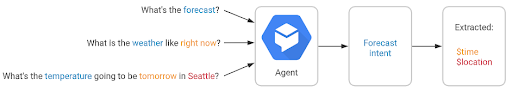
\includegraphics[width=0.85\textwidth]{inleiding-intent-entity}
    \caption{Schematische voorstelling van een intent met entities \autocite{GoogleCloud2020}}
\end{figure}

Intents worden ondersteund door (g)een of meerdere entities. Een entity is een soort parameter die door NLP uit de tekst wordt gehaald die dan gebruikt wordt om beter in te spelen op wat de gebruiker echt specifiek vraagt. In onderstaand voorbeeld zijn er entities voor de tijd en voor de locatie. Doordat er in de laatste zinnen extra informatie is toegevoegd in de tekst (tijd en locatie), kan de chatbot specifiek de weersvoorspelling tonen op een bepaald moment of op een specifieke plaats.

\subsection{Application Programming Interface (API)}
\label{subsec:begrippen-api}

Een Application Programming Interface (API) wordt gebruikt om twee applicaties te laten communiceren met elkaar. Een API is een toegangspunt die je kunt gebruiken om informatie op te vragen of om iets te wijzigen op een server. Een API gaat een verzoek ontvangen, doorsturen naar de server en uiteindelijk een antwoord terugsturen naar de gebruiker. API’s worden in deze bachelorproef gebruikt om vanuit de eigen geschreven code te communiceren met de servers van de verschillende platformen om chatbots te trainen en te testen. Meer informatie en uitleg omtrent API’s en de werking binnen dit onderzoek kan worden gevonden in sectie \ref{sec:automatisatie}.


\newpage
\section{\IfLanguageName{dutch}{Probleemstelling}{Problem Statement}}
\label{sec:probleemstelling}

Digital product studio In The Pocket heeft regelmatig projecten lopen waarbij het implementeren van een chatbot een meerwaarde kan zijn op het resultaat. Doordat In The Pocket partner is van Google Cloud, werken ze vooral met de producten die aangeboden worden door Google. Er zijn tal van platformen en tools beschikbaar voor het bouwen van chatbots en het is boeiend om te onderzoeken of het interessant zou zijn om over te stappen naar een ander platform om chatbots op te leveren die een lagere foutenmarge en beter begrijpend vermogen hebben. Dit moet onderzocht worden, omdat er een grote verscheidenheid aan platformen is en deze veranderen en evolueren continu. Ook de verschillende nieuwe ontwikkelingen binnen AI en ML hebben invloed op de prestaties van de verschillende platformen.

\section{\IfLanguageName{dutch}{Onderzoeksvraag}{Research question}}
\label{sec:onderzoeksvraag}

Binnen dit onderzoek zijn er 3 onderzoeksvragen te beantwoorden. Twee vragen kunnen beantwoord worden vanuit een vergelijkend onderzoek, de resterende vraag zal beantwoord worden door een experiment.
\begin{itemize}
    \item Welk NLP-platform heeft het beste begrijpend vermogen om de intentie van berichten correct te interpreteren ?
    \item Wat zijn de voordelen en tekortkomingen van de verschillende platformen ?
    \item Welk platform biedt de meeste integraties met andere diensten aan ?
\end{itemize}

\section{\IfLanguageName{dutch}{Onderzoeksdoelstelling}{Research objective}}
\label{sec:onderzoeksdoelstelling}

Het is de bedoeling om met dit onderzoek In The Pocket een beter actueel beeld te geven van de meest interessante platformen en hun eigenschappen. Ook is het de bedoeling dat er een NLP-platform wordt gekozen die de meest interessante keuze is. Daarbij is het begrijpend vermogen en een lage foutmarge prioriteit. Eigenschappen zoals integratiemogelijkheden, (programmeer) taalondersteuning, en prijs zijn ook doorslaggevend. Binnen dit onderzoek zullen er enkel gratis platformen bekeken en vergeleken worden. Deze bachelorproef kan in de toekomst ook nuttig.

\newpage
\section{\IfLanguageName{dutch}{Opzet van deze bachelorproef}{Structure of this bachelor thesis}}
\label{sec:opzet-bachelorproef}

% Het is gebruikelijk aan het einde van de inleiding een overzicht te
% geven van de opbouw van de rest van de tekst. Deze sectie bevat al een aanzet
% die je kan aanvullen/aanpassen in functie van je eigen tekst.

De rest van deze bachelorproef is als volgt opgebouwd:

In Hoofdstuk~\ref{ch:stand-van-zaken} wordt een overzicht gegeven van de stand van zaken binnen het onderzoeksdomein, op basis van een literatuurstudie.  Daarbij wordt er gekeken naar wat chatbots juist zijn, welke soorten er bestaan, wat de voor-en nadelen zijn, wat de mogelijke verbeteringen zijn, wat de toekomst kan/zal bieden en hoe het zit met de beveiliging. Daarnaast zal er ook uitleg worden voorzien over NLP en de subdomeinen NLU en NLG. Als laatste zullen de verschillende platformen kort theoretisch besproken en met elkaar vergeleken worden.

In Hoofdstuk~\ref{ch:methodologie} wordt het experiment toegelicht en worden de gebruikte onderzoekstechnieken besproken om een antwoord te kunnen formuleren op de onderzoeksvragen.

In Hoofdstuk~\ref{ch:resultaten}  zullen de resultaten van het experiment geanalyseerd, vergeleken en besproken worden.

In Hoofdstuk~\ref{ch:conclusie}, tenslotte, wordt de conclusie gegeven en een antwoord geformuleerd op de onderzoeksvragen.









